\documentclass{tokh}

\usepackage[colorlinks=true]{hyperref}

\newcommand{\cfbox}[2]{%
    \colorlet{currentcolor}{.}%
    {\color{#1}%
    \fbox{\color{currentcolor}#2}}%
}

\newlength{\currentparskip}
\newlength{\currentparindent}
\newenvironment{stdminipage}[1]
{\setlength{\currentparskip}{\parskip}%
  \setlength{\currentparindent}{\parindent}%
   \begin{minipage}[t]{#1}%
   \setlength{\parskip}{\currentparskip}%
   \setlength{\parindent}{\currentparindent}%
  }
  {\end{minipage}}

\usepackage{xspace}
\newcommand{\missionrule}[1]{\noindent\textbf{#1}\xspace}

\begin{document}
%\squelchbackground
%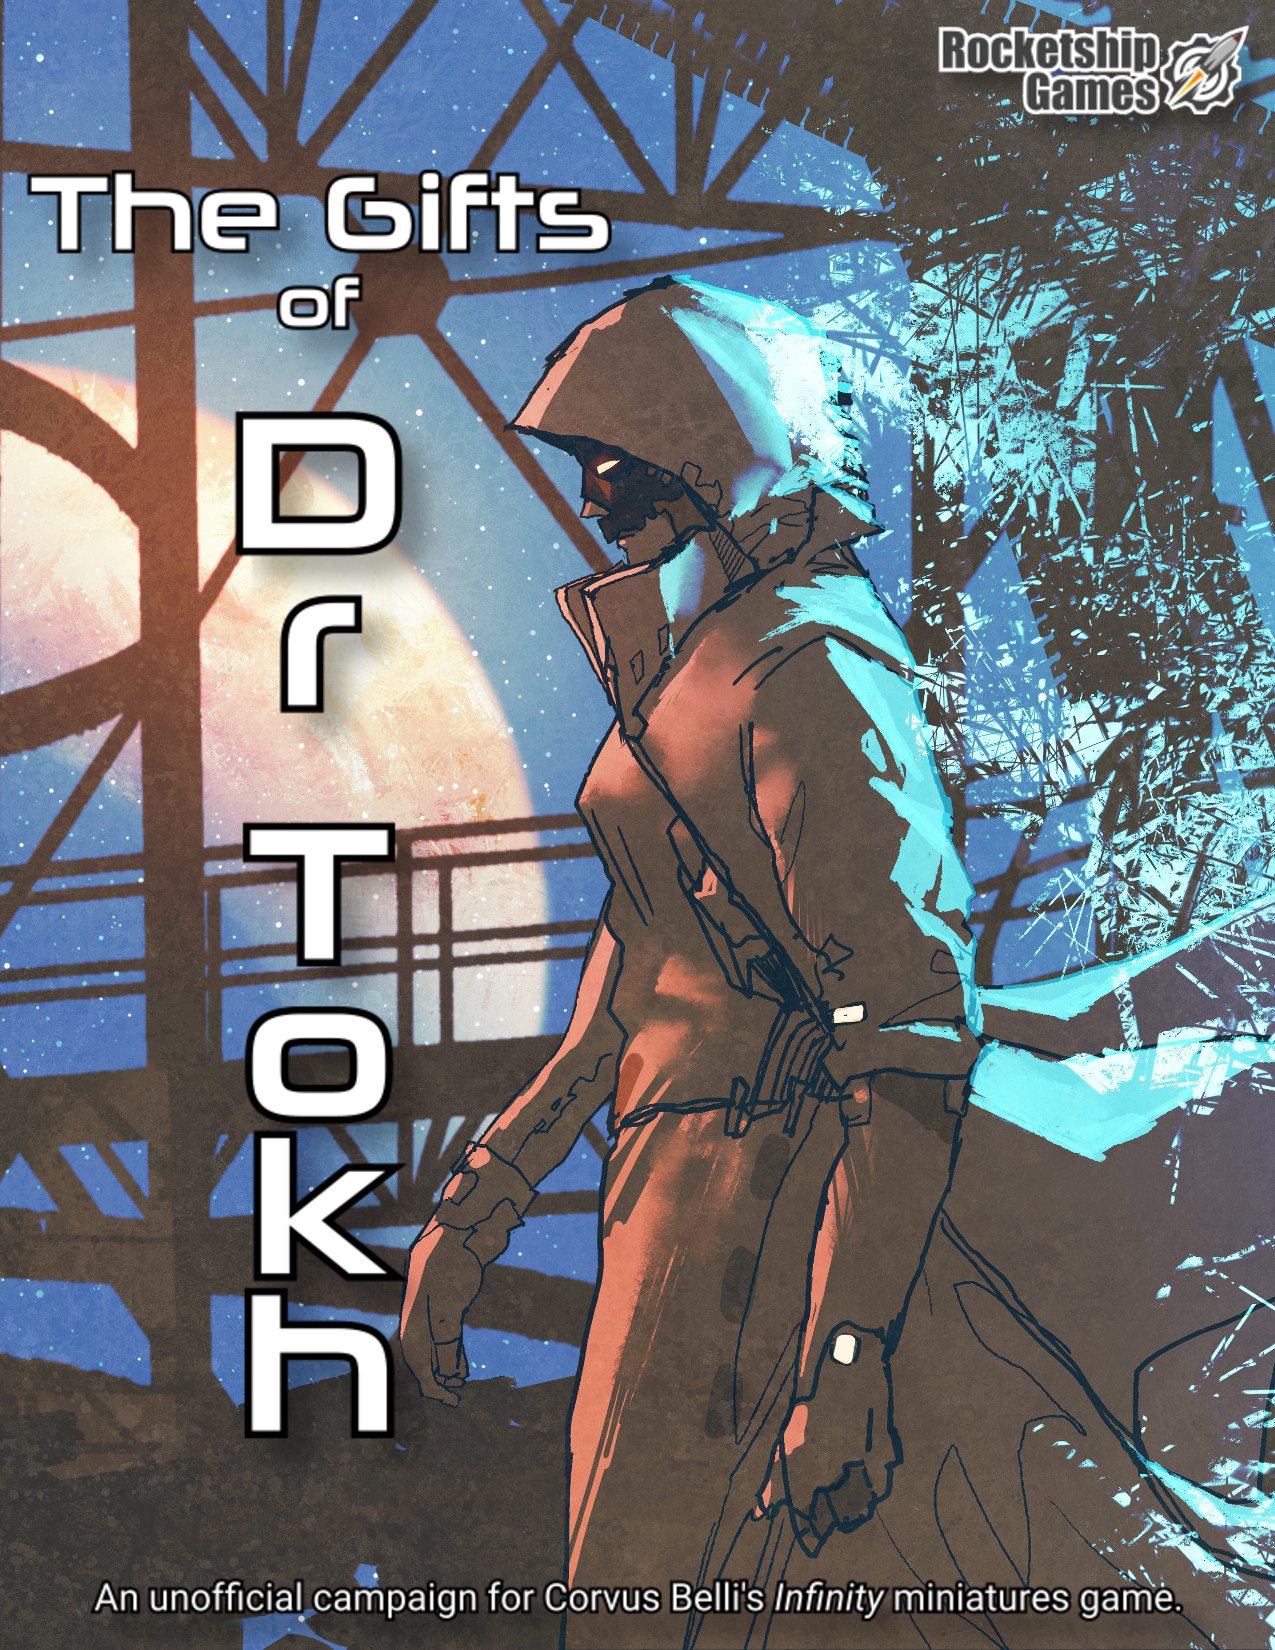
\includepdf[pages={1},fitpaper,offset=0cm 0cm]{art/cover/tokh-cover.pdf}
%\pagebreak
%\restorebackground

\chapter{Common Rules}

\missionrule{Initiative Roll.}  A standard Initiative Roll determines
Initiative and Deployment, except the Initiative Roll may be made
against either your Lieutenant or your Special Agent.  In addition, in
the Quadrant missions:

\begin{itemize}\shortlist
\item The player that chose the mission receives a +3 MOD.

\item Players whose alliance controls the associated Breach Point or
  Quadrant receive a~+3 MOD.
\end{itemize}

\missionrule{Connect Objective.} The Connect Objective short skill is
available in some missions:

% \vspace{-7pt}
\noindent\hfill
{\setlength\fboxrule{2pt}
\cfbox{LimeGreen}{\begin{minipage}{6.5in}
  \colorbox{LimeGreen}{\parbox{\linewidth-2\fboxsep}{\textcolor{White}{\textbf{\large Connect Objective} \hfill Short Skill}}}\\
  \colorbox{SkyBlue}{\parbox{\linewidth-2\fboxsep}{\textcolor{White}{Attack}}}

  \medskip
  \textsc{Requirements}
  \begin{squishitemize}
  \item The user must be a model (not a marker) in base contact with a
    designated objective.
  \end{squishitemize}

  \medskip
  \colorbox{Gray!24}{\begin{minipage}{\linewidth-2\fboxsep}

  \medskip      
      \textsc{Effects}
      \begin{squishitemize}
      \item The user makes a Normal WIP roll with a~-3 MOD to attempt
        connecting the objective.  \emph{Specialist Troops
          automatically pass this roll.}

      \item If successful, the acting player connects to the objective
        (mark it appropriately) and the other player is no longer
        connected if they previously were (remove any marker).
      \end{squishitemize}
    \end{minipage}}
\end{minipage}}}
\hfill\hbox to 0pt{}

\medskip
\missionrule{Network Terminals.}  The Connect Objective short skill
may be applied to Network Terminals in all missions.  At the end of
each game round, if a player has a Specialist Troop model (not a
marker) in base contact with a Network Terminal they have connected,
and no enemy troops are in base contact, the player receives a Network
Directory token.  If that troop is their Special Agent, they receive
two tokens.

\missionrule{Experience.}  After each mission, your Special Agent is
permanently improved by choosing from:

\begin{itemize}\shortlist
\item +1 to one of CC, BS, PH, or WIP
\item +1 to MOV (first value)
\item +1 to ARM (once per campaign)
\item +1 to BTS (once per campaign)
\end{itemize}

If you won and the Lieutenant listed on your army list survived, their
CC, BS, PH, or WIP may be permanently improved by~+1.  You may not
improve a single attribute for any given Lieutenant more than once per
campaign (e.g., after two victorious missions they could not have
improved BS twice).
  
If you lost the mission, you receive a Karma token.  If you lost by~7
or more objective points then you receive two Karma tokens.  Karma
tokens may be discarded at any point in a later mission to reroll a
single die of yours.  You may not reroll a die that has already been
rerolled.

\chapter{Mission: Breach Point}

\emph{\emph{Breach Point} is a RECON+ mission played on a~2'x3' play area.}

\section{Play Area}
\vspace{-2\parskip}
\noindent\begin{stdminipage}{\linewidth-(2in+1.5em)}
\vspace{0pt}   
\noindent
Whichever player takes Deployment in the Initiative Roll chooses
either of the long edges of the play area as the Breach Point.

There is an Exclusion Zone extending~6'' out along the full extent of
the Breach Point edge.

The Deployment Zones are clipped triangles along the short edges
stretching from~3'' forward of that edge along the inner Exclusion
Zone boundary, to the point~12'' forward on the opposite edge of the
play area (this may also be measured by stretching a line from the
corner inside the Exclusion Zone to a point~12'' forward on the far
play area edge, with no models permitted to be deployed inside the
Exclusion Zone).

There are two scoring Sectors: The Target Sector, extending~6'' from
the Breach Point edge and~4'' on either side of the short centerline;
and the Approach Sector, extending~12'' from the Breach Point edge
and~9'' on either side of the short centerline but excluding the
Target Sector.

A Network Terminal is placed on the short center axis of the
table,~4'' from the long play area edge opposite the Breach Point
edge.
\end{stdminipage}
\hfill
\begin{minipage}[t]{2in}\centering
\vspace{4pt}   
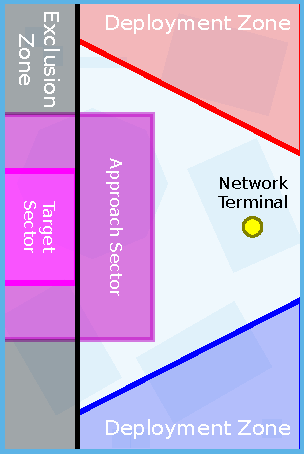
\includegraphics{maps/map-breachpoint}

\medskip\small%
\emph{(flip if opposite long edge chosen as the Breach Point)}
\end{minipage}

\section{Mission Rules}

Special Agents count as an additional 30 army points for purposes of
calculating domination.

\section{Scoring}

Players may score up to~10 objective points via the following
conditions at game end:
\begin{itemize}\shortlist
\item 1pt for having a model with more than half its base inside the
  Approach Sector.
\item 2pts for dominating the Approach Sector.
\item 2pt for having a model with more than half its base inside the
  Target Sector.
\item 3pts for dominating the Target Sector.
\item 1pt if the opposing Special Agent is in a Null state or eliminated.
\item 1pt if more points of the opposing army list have been destroyed.
\end{itemize}

\vfill
\vbox to 0pt{}
\chapter{Mission: Cyber}

\emph{\emph{Cyber} is a RECON+ mission in which the alliances attempt
  to penetrate the Cyber-Informatics Laboratory and download
  revolutionary digital viruses and artificial intelligence kernels.}


\section{Play Area}
\vspace{-2\parskip}
\noindent\begin{stdminipage}{\linewidth-(2in+1.5em)}
\vspace{0pt}   
\noindent
The Deployment Zones are~6'' areas along the short
play area edges.

Four Consoles are placed in a grid, each~6'' from a long edge of the
play area and~8'' from a deployment zone.

A Network Terminal is placed at the center of the play area.

\section{Mission Rules}

The Connect Objective short skill may be applied to Consoles in this
mission.  The Consoles are Repeaters for the Hackers of both players.
They do not apply Firewall MODs.

\end{stdminipage}
\hfill
\begin{minipage}[t]{2in}\centering
\vspace{4pt}   
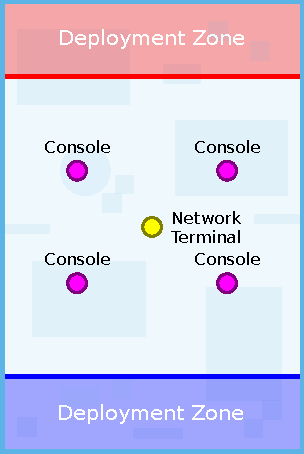
\includegraphics{maps/map-cyber}
\end{minipage}

\section{Scoring}

Players may score up to~10 objective points via the following
conditions at game end:
\begin{squishitemize}
\item 1pt for each Console closest to your Deployment Zone connected.
\item 2pts for each Console farthest from your Deployment Zone
  connected.
\item 2pts for having your Special Agent in base contact with a
  connected Console.
\item 1pt if the opposing Special Agent is in a Null state or eliminated.
\item 1pt if more points of the opposing army list have been destroyed.
\end{squishitemize}

\vfill
\vbox to 0pt{}
\chapter{Mission: Bio/Xeno}

\emph{\emph{Bio/Xeno} is a RECON+ mission in which the alliances
  attempt to harvest experimental lifeforms crafted by Dr.~Tokh, some
  of the more dangerous of which have escaped amid the fighting!}

\section{Play Area}
\vspace{-2\parskip}
\noindent\begin{stdminipage}{\linewidth-(2in+1.5em)}
\vspace{0pt}   
\noindent
The Deployment Zones are~6'' areas along the short play area edges.

There is an Exclusion Zone extending~6'' on either side of the short
centerline of the play area~(12'' total, across the whole board).

%There is an Exclusion Zone extending~6'' on both sides of the short
%centerline of the play area (12'' across total) and covering the full
%extent between long edges.

Place two Stasis Chambers on the short centerline of the play area,
each~5'' from the center toward a different long edge~(10'' apart).

Before any deployment begins, the player with Deployment places a
Network Terminal adjacent to either long edge on the short centerline.

\vspace*{-8pt}
\section{Mission Rules}

\vspace*{-4pt}
As part of their deployment, each player places two Xenomorphs in
Hidden Deployment within the Exclusion Zone in their opponent's half
of the play area.  These do not join their army lists and are
considered enemies to both players.  The reactive player
controls all revealed Xenomorphs and may choose to ARO with the
unrevealed Xenomorphs they placed.

\noindent\begin{minipage}{\linewidth}\center
\setlength\fboxrule{2pt}  
\cfbox{Dandelion}{\begin{minipage}{5in}
    \colorbox{Dandelion}{\parbox{\linewidth-2\fboxsep}{\textbf{\textcolor{White}{Xenomorph}}}}

\colorbox{Gray!24}{\begin{minipage}{\linewidth-2\fboxsep}

    \medskip    
\noindent\hfill\begin{tabular}[t]{ccccccccc}
\rowcolor{Black}  \textbf{\textcolor{White}{MOV}} & \textbf{\textcolor{White}{CC}} & \textbf{\textcolor{White}{BS}} & \textbf{\textcolor{White}{PH}} & \textbf{\textcolor{White}{WIP}} & \textbf{\textcolor{White}{ARM}} & \textbf{\textcolor{White}{BTS}} & \textbf{\textcolor{White}{W}} & \textbf{\textcolor{White}{S}}\\
  \hline
  6-4 & 22 & 8 & 15 & 10 & 0 & 3 & 1 & 2\\
\end{tabular}
\hfill\hbox to 0pt{}

\medskip
Hyper-Dynamics L1, Kinematika L2, Sixth Sense L2, Superjump\\
BS Weapons: \emph{---}\hfill CC Weapons: \emph{Viral CCW}
    \end{minipage}}
\end{minipage}}
\end{minipage}

\end{stdminipage}
\hfill
\begin{minipage}[t]{2in}\centering
\vspace{4pt}   
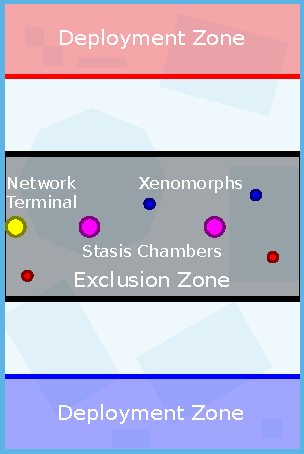
\includegraphics{maps/map-bio}

\medskip\small%
\emph{(Network Terminal may be on opposite long edge)}


%\begin{minipage}[t]{1in}
%  \raisebox{-.95in}[0pt][0pt]{
\smallskip
\centerline{
\includegraphics[height=1.1in]{art/icons/xeno}}
%\end{minipage}%

\end{minipage}

\medskip%
Also as part of deployment, three troopers in each player's army are
given Adhesive Launchers.

The Connect Objective short skill may be applied to Stasis Chambers.

\vspace*{-8pt}
\section{Scoring}

\vspace*{-4pt}
Players may score up to~10 objective points via the following
conditions at game end:
\begin{squishitemize}
\item 1pt for having connected a Stasis Chamber at any point in the game.
\item 2pt for each Stasis Chamber you have connected.
\item 2pts for having at least one model in base contact with a
  Xenomorph in Immobilized state;\\
  OR 1pt for having at least one model in base contact with a
  Xenomorph in Unconscious state.
%\item 1pt for having a second model in base contact with a
%  second Immobilized or Unconscious Xenomorph;\\
\item 2pt if your Special Agent is in base contact with an
  Immobilized or Unconscious Xenomorph.

% \item 1pt if the opposing Special Agent is in a Null state or eliminated.
\item 1pt if more points of the opposing army list have been destroyed.
\end{squishitemize}

\vfill
\vbox to 0pt{}

\chapter{Mission: MechE}

\chapter{Mission: Plant}

% played on a~2'x3' play area as

\emph{\emph{Plant} is a RECON+ mission in which the alliances attempt
  to destroy the campus physical plant using explosives chosen to
  incriminate their opponents, while preventing being similarly
  implicated themselves.}


\section{Play Area}
\vspace{-2\parskip}
\noindent\begin{stdminipage}{\linewidth-(2in+1.5em)}
\vspace{0pt}   
\noindent
Whichever player takes Deployment in the Initiative Roll chooses a
corner of the play area for their Deployment Zone, from which the
latter extends~12'' out.  The other player takes the diagonally
opposite corner as their Deployment Zone, again up to~12'' out.

A Network Terminal is placed at the center of the play area.

\section{Mission Rules}
As part of their deployment, both players secretly choose and record~3
scenery pieces wholly within~24'' of their opponent's Deployment Zone
corner as Vulnerable Infrastructure.  Each piece must have a footprint
of at least~4 square inches (e.g., a 2''x2'' square or~2.5'' diameter
circle).

In addition, as part of deployment, three troopers in each player's
army are given D-Charges.  This is public information as usual.
D-Charges already included in troopers' profiles may also be used.

\end{stdminipage}
\hfill
\begin{minipage}[t]{2in}\centering
\vspace{4pt}   
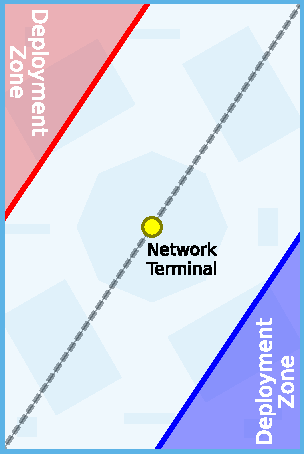
\includegraphics{maps/map-plant}
\end{minipage}

\section{Scoring}

Players may score up to~10 objective points via the following
conditions:
\begin{itemize}\shortlist
\item 1pt for each D-Charge you place on your chosen Vulnerable
  Infrastructure.
\item 1pt for each D-Charge you detonate on your chosen Vulnerable
  Infrastructure.
\item 3pts if you detonate D-Charges on all of your chosen Vulnerable
  Infrastructure simultaneously.

\item 1pt if the opposing Special Agent is in a Null state or
  eliminated at game end.
\end{itemize}

\vfill
\vbox to 0pt{}

\chapter{Mission: Datacenter}

\emph{\emph{Datacenter} is a doubles team mission on a~4'x4' play area
  and with~300 army points per side in which the alliances attempt to
  secure Dr Tokh's most valuable data from a major campus computing
  cluster.}

\section{Play Area}

The Deployment Zones are~12'' areas along opposing play area edges.

Nine Server objectives are placed in a grid: Three on the centerline
between the deployment zones, one at the center and the other two~12''
from each edge; and six in two lines of three~8'' from that centerline
in each half of the play area, each with one at the center and the
other two~12'' from each edge.

Each Server is randomly assigned a Data Topic without it being
revealed to either player, via markers placed facedown next to them.
There are three each of three Data Topics: Bio/Xeno, Cyber, and MechE.

\section{Mission Rules}

The standard Initiative Roll may be made against any of your team's
Lieutenants or Special Agents.  Teams whose alliance controls more
Quadrants than their opponents' receive a~+3 MOD to this roll.

%  \href{http://wiki.infinitythegame.com/en/index.php?title=Initiative_and_Deployment}{}

The Connect Objective short skill may be applied to Servers in this
mission.

Players may look at the assigned Data Topic for any Server they have
connected at any time.  In addition, Network Directory tokens earned
by players in the preceding missions may be discarded to look at the
assigned Data Topic for up to~3 Servers per token.  In neither case
are the Data Topics revealed to the other player.  Players may keep
secret notes about what they have learned of the Servers.


\section{Scoring}

Players may score up to~20 objective points via the following
conditions at game end:
\begin{squishitemize}
\item 1pt for each Data Topic of which the player is connected to at
  least one Server.
\item 2pts for each Data Topic of which the player is connected to the
  most Servers.
\item 1pt for being connected to at least one Server for each of the
  three Data Topics.

\item 2pts for each friendly Special Agent in base contact with a
  Server (connected or otherwise).
\item 2pts for each friendly Special Agent wholly in the enemy half of the
  play area.
\item 1pt for each opposing Special Agent in a Null State or eliminated.

% \item 1pt if at least~50\% of your army list by points has survived.
%\item 1pt if more points of the opposing army list have been destroyed.
\end{squishitemize}


\end{document}
